\chapter{Complex numbers}
The equation $x^2 + 1 = 0$ has no solution in $\mathbb{R}$. To solve this problem, we introduce a new number $i$ such that $i^2 = -1$. The set of complex numbers is defined as follows. \\
\begin{proof}
    Let's prove that the equation $x^2 + 1 = 0$ has no solution in $\mathbb{R}$.
\end{proof}

\section{Definition and properties of complex numbers}
\begin{definition}[Complex numbers]
    The set of complex numbers is defined as $\mathbb{C} = \{ a + bi \mid a, b \in \mathbb{R} \}$ where $i$ is the imaginary unit with the property that $i^2 = -1$. Addition and mutliplication of complex numbers are defined as follows:
    \begin{itemize}[itemsep=1pt,label=$\circ$]
        \item $(a + bi) + (c + di) = (a + c) + (b + d)i$
        \item $(a + bi)(c + di) = (ac - bd) + (ad + bc)i$
    \end{itemize}
\end{definition}
Let also add that:
\begin{itemize}[itemsep=1pt,label=$\circ$]
    \item $\exists 0 \in \mathbb{C}: 0 = 0 + 0i$ such as $(a + bi) + (0 + 0i) = (a + bi) \quad \forall a, b \in \mathbb{R}$.
    \item $\exists$ an inverse for $(a + bi): ((-a) + (-b)i) + (a + bi) = 0 + 0i = 0 \quad \forall a, b \in \mathbb{R}$.
    \item $\exists 1 \in \mathbb{C}: 1 = 1 + 0i$ such as $(a + bi)(1 + 0i) = (a + bi) \quad \forall a, b \in \mathbb{R}$.
    \item $\forall z \in \mathbb{C} : z \neq 0 \implies \exists z^{-1} \in \mathbb{C} : z z^{-1} = 1$.
\end{itemize}

\begin{definition}[Inverse of a complex number]
    Let $z = a + bi \in \mathbb{C}$ such as $z \neq 0$ (i.e., $a^2 + b^2 \neq 0$). The inverse of $z$ is given by:
    \[
        z^{-1} = \frac{a}{a^2 + b^2} - \frac{b}{a^2 + b^2}i
    \]
\end{definition}
Let's verify that $z z^{-1} = 1$:
\[
    z z^{-1} = (a + bi) \left( \frac{a}{a^2 + b^2} - \frac{b}{a^2 + b^2}i \right) = \frac{a^2 + b^2}{a^2 + b^2} = 1
\]
\begin{eg}
    Let's verify that complex numbers respect the distributive property. \\ Let $z_1 = (a_1 + b_1 i)$, $z_2 = (a_2 + b_2 i)$ and $z_3 = (a_3 + b_3 i)$ be three complex numbers. We want to show that:
    \[
        z_1(z_2 + z_3) = z_1 z_2 + z_1 z_3
    \]
    Let's compute left side:
    \[
        z_1(z_2 + z_3) = (a_1 + b_1 i)((a_2 + a_3) + (b_2 + b_3)i)
    \]
    \[
        = (a_1(a_2 + a_3) - b_1(b_2 + b_3)) + (a_1(b_2 + b_3) + b_1(a_2 + a_3))i
    \]
    Now, let's compute the right side:
    \[
        z_1 z_2 + z_1 z_3 = (a_1 a_2 - b_1 b_2 + a_1 a_3 - b_1 b_3) + (a_1 b_2 + b_1 a_2 + a_1 b_3 + b_1 a_3)i
    \]
    Both sides are equal, thus $\mathbb{C}$ is a commutative field.
\end{eg}
We can prove that $\mathbb{C}$ is not an ordered field. Indeed, if we assume that $i > 0$, then $i^2 = -1 > 0$ which is a contradiction. If we assume that $i < 0$, then $-i > 0$ and $(-i)^2 = -1 > 0$ which is also a contradiction. Thus, $\mathbb{C}$ is not an ordered field.

\section{Form of complex numbers}
Complex numbers can be represented in 3 different forms.
\subsection{Algebraic form}
\begin{definition}[Algebraic form]
    The algebraic form of a complex number $z = a + bi$ where $a, b \in \mathbb{R}$. Which can also be written as:
    \[
        z = \text{Re}(z) + \text{Im}(z)i
    \]
    where $\text{Re}(z) = a$ is the real part of $z$ and $\text{Im}(z) = b$ is the imaginary part of $z$.
\end{definition}
The modulus of a complex number $z = a + bi$ is defined as:
\[
    |z| = \sqrt{(\text{Re} (z))^2 + (\text{Im} (z))^2} = \sqrt{a^2 + b^2} \geq 0
\]
\[
    |z| = 0 \iff z = 0
\]

\subsection{Trigonometric form}
\begin{definition}[Trigonometric form]
    The trigonometric form of a complex number $z = a + bi$ is given by:
    \[
        z = r(\cos(\theta) + i \sin(\theta)) \quad r \geq 0, \theta \in \mathbb{R}
    \]
    where:
    \begin{center}
        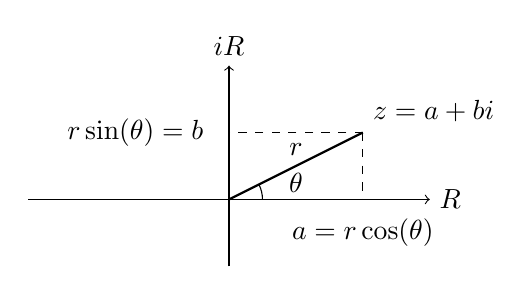
\begin{tikzpicture}[scale=.85]
            \draw[->] (-3,0) -- (3,0) node[right] {$\mathbb{R}$};
            \draw[->] (0,-1) -- (0,2) node[above] {$i \mathbb{R}$};
            \draw[thick] (0,0) -- (2,1) node[above right] {$z = a + bi$};
            \draw[dashed] (2,1) -- (2,0);
            \draw[dashed] (2,1) -- (0,1);
            \draw (0.5,0) arc[start angle=0,end angle=26.57,radius=0.5];
            \node at (1,0.25) {$\theta$};
            \node at (1,.75) {$r$};
            \node at (2,-0.5) {$a = r \cos(\theta)$};
            \node at (-1.4,1) {$r \sin(\theta) = b$};
        \end{tikzpicture}
    \end{center}
    and:
    \[
        \text{Re}(z) = a = r \cos(\theta), \quad \text{Im}(z) = b = r \sin(\theta)
    \]
\end{definition}
$\newline$ %space error
The modulus of $z$ is given by:
\[
    |z| = r = \sqrt{r^2 \cos^2(\theta) + r^2 \sin^2(\theta)} = r \geq 0
\]
The argument of $z$ ($z \neq 0$) is given by:
\[
    r \neq 0 \implies \sin(\theta) = \frac{\text{Im}(z)}{r}, \quad \cos(\theta) = \frac{\text{Re}(z)}{r}
\]
Showing that $\theta$ is defined up to an additive factor of $2k\pi$, $k \in \mathbb{Z}$. Also:
\[
    \tan(\theta) = \frac{\text{Im}(z)}{\text{Re}(z)} = \frac{b}{a} \quad \text{if } a \neq 0
\]
\begin{eg}
    Let's find the argument of $z = a + bi$. We have: \\
    If $a > 0$, then:
    \[
        \theta = \arctan\left(\frac{b}{a}\right) + 2k\pi, \quad k \in \mathbb{Z}
    \]
    \begin{center}
        \begin{tikzpicture}[scale=.85]
            \draw[->] (-3,0) -- (3,0) node[right] {$\mathbb{R}$};
            \draw[->] (0,-1) -- (0,2) node[above] {$i \mathbb{R}$};
            \draw[thick] (0,0) -- (2,1);
            \draw[dashed,color=primary] (2,1) -- (2,0);
            \draw[dashed,color=primary] (2,1) -- (0,1);
            \draw[->,primary] (0.5,0) arc[start angle=0,end angle=26.57,radius=0.5];
            \node[primary] at (2,0.25) {$\theta = \text{arg}(z)$};
            \node[primary] at (2,-0.3) {$a$};
            \node[primary] at (-0.4,1) {$b$};
        \end{tikzpicture}
    \end{center}
    If $a < 0$, then:
    \[
        \theta = \arctan\left(\frac{b}{a}\right) + (2k + 1)\pi, \quad k \in \mathbb{Z}
    \]
    \begin{center}
        \begin{tikzpicture}[scale=.85]
            \draw[->] (-3,0) -- (3,0) node[right] {$\mathbb{R}$};
            \draw[->] (0,-2) -- (0,2) node[above] {$i \mathbb{R}$};

            \draw[thick,secondary] (0,0) -- (2,1);
            \draw[->,secondary] (0.5,0) arc[start angle=0,end angle=25,radius=0.5];
            \node[secondary] at (2.8,0.6) {$\theta \neq \arctan\frac{b}{a}$};

            \draw[thick] (0,0) -- (-2,-1);
            \draw[dashed,primary] (-2,-1) -- (-2,0);
            \draw[dashed,primary] (-2,-1) -- (0,-1);
            \draw[->,primary] (0.7,0) arc[start angle=0,end angle=205,radius=0.7];
            \node[primary] at (-2.3,0.8) {$\arctan\frac{b}{a} + \pi = \theta$};
            \node[primary] at (-2,0.3) {$a$};
            \node[primary] at (0.4,-1) {$b$};
        \end{tikzpicture}
    \end{center}
    Finally, if $a = 0$, then:
    \[
        \theta = \begin{cases}
            \frac{\pi}{2} + 2k\pi, & b > 0 \\
            \frac{3\pi}{2} + 2k\pi, & b < 0 \\
        \end{cases}
    \]
    \begin{center}
        \begin{tikzpicture}[scale=.85]
            \draw[->] (-3,0) -- (3,0) node[right] {$\mathbb{R}$};
            \draw[->] (0,-2) -- (0,2) node[above] {$i \mathbb{R}$};

            \draw[thick,secondary] (0,0) -- (0,1.5);
            \draw[->,secondary] (0.5,0) arc[start angle=0,end angle=90,radius=0.5];
            \node[secondary] at (0.3, 1.5) {$z$};
            \node[secondary] at (1.2,0.5) {$\theta = \frac{\pi}{2}$};

            \draw[thick,primary] (0,0) -- (0,-1.5);
            \draw[->,primary] (0.7,0) arc[start angle=0,end angle=270,radius=0.7];
            \node[primary] at (-0.3, -1.5) {$z$};
            \node[primary] at (-1.5,-0.5) {$\theta = \frac{3\pi}{2}$};
        \end{tikzpicture}
    \end{center}
\end{eg}
$\newline$ %space error
The argument of $z$ is only defined for $z \neq 0$.

\subsection{Exponential form}
\begin{definition}[Exponential form]
    The exponential form of a complex number $z = a + bi$ is given by:
    \[
        e^z = \text{exp}(z) = e^a (\cos(b) + i \sin(b))
    \]
    If $z = a$, then:
    \[
        e^z = e^a (\cos(0) + i \sin(0)) = e^a (1 + 0) = e^a
    \]
    If $z = bi$, then:
    \[
        e^z = e^0 (\cos(b) + i \sin(b)) = e^{ib}
    \]
\end{definition}

\begin{definition}[Euler's formula]
    For any real number $\theta \in \mathbb{R}$, we have:
    \[
        e^{i\theta} = \cos(\theta) + i \sin(\theta)
    \]
\end{definition}
Let's show that $e^{i(\theta_1 + \theta_2)} = e^{i\theta_1} \cdot e^{i\theta_2}$:
\[
    e^{i(\theta_1 + \theta_2)} = \cos(\theta_1 + \theta_2) + i \sin(\theta_1 + \theta_2)
\]
\[
    = (\cos(\theta_1) \cos(\theta_2) - \sin(\theta_1) \sin(\theta_2)) + i (\sin(\theta_1) \cos(\theta_2) + \cos(\theta_1) \sin(\theta_2))
\]
\[
    = (\cos(\theta_1) + i \sin(\theta_1))(\cos(\theta_2) + i \sin(\theta_2)) = e^{i\theta_1} \cdot e^{i\theta_2}
\]
Let's also show that an imaginary exponential is periodic with period $2\pi$:
\[
    y_1 = y_2 + 2k\pi, \ k \in \mathbb{Z} \implies e^{i y_1} = e^{i y_2 + 2k\pi} = e^{i y_2}(\cos(2k\pi) + i \sin(2k\pi)) = e^{i y_2}
\]
If we take a complex number in trigonometric form $z = r(\cos(\theta) + i \sin(\theta))$, we can write it in exponential form as:
\[
    z = r e^{i\theta}
\]

\subsection{Summary of the forms of a complex number}
A complex number can be represented as:
\begin{align*}
    z &= \text{Re}(z) + i \cdot \text{Im}(z) &\text{(Algebraic form)} \\
    &= |z|(\cos(\text{arg}(z)) + i \sin(\text{arg}(z))) &\text{(Trigonometric form)} \\
    &= |z| e^{i \text{arg}(z)} &\text{(Exponential form)} \\
\end{align*}
Usually complex numbers are represented in polar form (trigonometric or exponential form).
\begin{eg}
    Let's show that the modulus of $z = e^{(e^{i \phi})}$ is equal to $e^{\cos(\phi)}$.
    \[
        z = e^{(e^{i \phi})} = e^{(\cos(\phi) + i \sin(\phi))} = e^{\cos(\phi)} e^{i \sin(\phi)} = e^{\cos(\phi)} \cdot (\cos(\sin(\phi)) + i \sin(\sin(\phi)))
    \]
    Thus, the modulus of $z$ is:
    \[
        |z| = \sqrt{(e^{\cos(\phi)})^2 \cdot [(\cos(\sin(\phi)))^2 + (\sin(\sin(\phi)))^2]} = e^{\cos(\phi)}
    \]
\end{eg}

\begin{eg}
    Let's find the exponential form of $z = -1 + i$. We need to calculate the modulus and the argument of $z$:
    \[
        |z| = \sqrt{(-1)^2 + 1^2} = \sqrt{2}
    \]
    Since $\text{Re}(z) = -1 < 0$ and $\text{Im}(z) = 1 > 0$, we are in the second case of the argument calculation:
    \[
        \theta = \arctan\left(\frac{1}{-1}\right) + \pi = -\frac{\pi}{4} + \pi = \frac{3\pi}{4}
    \]
    Thus, the exponential form of $z$ is:
    \[
        z = \sqrt{2} e^{i \frac{3\pi}{4}}
    \]
\end{eg}

\begin{eg}
    Let's find the algebraic form of $z = 5 e^{i \frac{2\pi}{3}}$. We have:
    \[
        z = 5 \left( \cos\left(\frac{2\pi}{3}\right) + i \sin\left(\frac{2\pi}{3}\right) \right) = 5 \left( -\frac{1}{2} + i \frac{\sqrt{3}}{2} \right) = -\frac{5}{2} + i \frac{5\sqrt{3}}{2}
    \]
\end{eg}

\subsection{Operations in polar form}
Polar form is very useful to perform operations on complex numbers.
\begin{definition}[Mutiplication in polar form]
    To multiply two complex numbers in polar form, we multiply their moduli and add their arguments. If $z_1 = r_1 e^{i \theta_1}$ and $z_2 = r_2 e^{i \theta_2}$, then:
    \[
        z_1 z_2 = r_1 r_2 e^{i (\theta_1 + \theta_2)}
    \]
\end{definition}
\begin{proof}
    Let $z_1 = r_1 e^{i \theta_1}$ and $z_2 = r_2 e^{i \theta_2}$. We have:
    \[
        z_1 z_2 = r_1 e^{i \theta_1} \cdot r_2 e^{i \theta_2}
    \]
    By using the property of exponentials, we get:
    \[
        z_1 z_2 = r_1 r_2 e^{i (\theta_1 + \theta_2)}
    \]
\end{proof}

\begin{eg}
    Let $z = e^{i \phi}$, $w = e^{i \psi}$, $|z| = 1$ and $|w| = 1$. Then:
    \[
        z w = e^{i(\phi + \psi)}
    \]
\end{eg}

\begin{definition}[Division in polar form]
    To divide two complex numbers in polar form, we divide their moduli and subtract their arguments. If $z_1 = r_1 e^{i \theta_1}$ and $z_2 = r_2 e^{i \theta_2}$, then:
    \[
        \frac{z_1}{z_2} = \frac{r_1}{r_2} e^{i (\theta_1 - \theta_2)} \quad \text{if } z_2 \neq 0
    \]
\end{definition}

\begin{definition}[Inverse in polar form]
    The inverse of a complex number, $z \neq 0$ in polar form is given by:
    \[
        z^{-1} = \frac{1}{r} e^{-i \theta} \quad \text{if } z = r e^{i \theta} \text{ and } r > 0
    \]
\end{definition}
\begin{proof}
    Let $z = r e^{i \theta}$ such that $r > 0$. We have:
    \[
        z z^{-1} = r e^{i \theta} \cdot \frac{1}{r} e^{-i \theta} = 1 \cdot e^{i(\theta - \theta)} = 1 \cdot e^0 = 1
    \]
\end{proof}

\begin{definition}[De Moivre's theorem]
    For any complex number $z = r e^{i \theta}$ and any integer $n \in \mathbb{N}^*$, we have:
    \[
        z^n = r^n e^{i n \theta} = r^n (\cos(n \theta) + i \sin(n \theta))
    \]
\end{definition}
\begin{proof}
    Let's prove this by induction. For $n = 1$, we have:
    \[
        z^1 = r^1 e^{i \cdot 1 \cdot \theta} = r e^{i \theta}
    \]
    Now, let's assume it's true for $n = k$, i.e., $z^k = r^k e^{i k \theta}$. For $n = k + 1$, we have:
    \[
        z^{k+1} = z^k z = (r^k e^{i k \theta})(r e^{i \theta}) = r^k r e^{i k \theta} e^{i \theta} = r^{k+1} e^{i (k+1) \theta}
    \]
    Thus, by induction, the theorem holds for all $n \in \mathbb{N}^*$.
\end{proof}

\subsection{The Most Beautiful Formula in Mathematics}
Let $y = \pi$, then:
\[e^{i\pi} = \cos(\pi) + i \sin(\pi) = -1 + 0 = -1\]
\begin{theorem}[Euler's identity]
    \[e^{i\pi} + 1 = 0
    \]
\end{theorem}
This formula links the 5 most important constants in mathematics: $e, i, \pi, 1, 0$.

\section{Exercices} % week 2 assignement
This section gathers a selection of exercises related to Chapter \thechapter, taken from weekly assignments, past exams, textbooks, and other sources. The origin of each exercise will be indicated at its beginning.